\section{Neural network implementation}
\subsection{Architecture}
A {\it mhcflurry} predictor consists of a embedding layer which transforms each amino acid to a learned vector representation, followed by a single hidden layer and finally a scalar output (figure \ref{fig:architecture}). We map IC50 concentrations onto a regression target between 0.0 and 1.0 using the same scheme as NetMHC: $y = 1.0 - max(1.0, log_{50000}(IC50))$.

\begin{figure}[h]
\centering
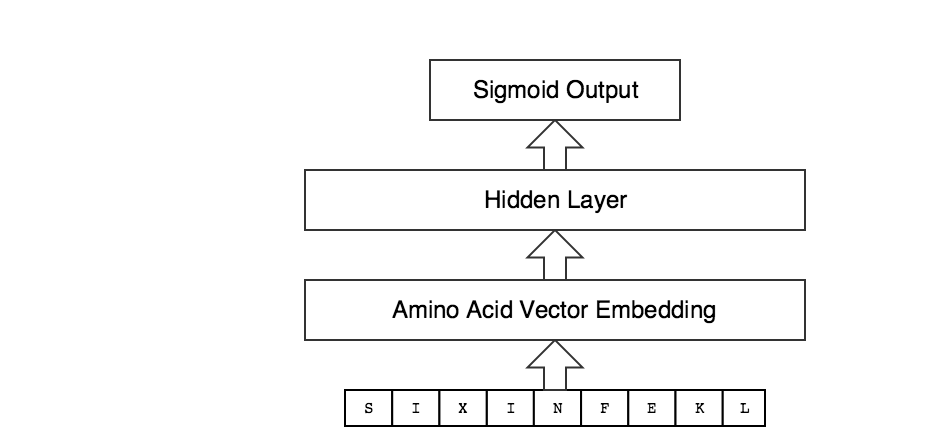
\includegraphics[scale=0.5]{figures/mhcflurry-gliffy-network.png}
\caption{Neural network architecture for predicting peptide-MHC affinities from fixed length amino acid sequences}
\label{fig:architecture}
\end{figure}

\subsection{Transforming all peptide lengths into a 9mer encoding}
Like NetMHC\cite{lundegaard2008accurate}, the mhcflurry predictor assumes length-9 peptides and uses an averaging scheme to reduce non-9mer peptides to a 9mer prediction task. Each non-9mer is mapped into multiple 9mer query peptides, and the predicted affinity is taken to be the geometric mean of the predictions for the queries. For 8mers, the query peptides are generated by inserting a sentinel ``X'' at every position in the sequence. For peptides longer than 9 amino acids, 9mers are generated by removing consecutive stretches of residues at every position. This scheme is also used for training, with the affinity of each query peptide set equal to the measured affinity of the non-9mer peptide it was generated from, and its weight adjusted so each measurement receives equal contribution.

\section{Pretraining a neural network with imputed training data}

